\documentclass{sig-alternate}
\usepackage{txfonts}
\usepackage[utf8]{inputenc}
\usepackage{array}
\usepackage{graphicx}
\usepackage{url}
\usepackage{caption}
\usepackage{subcaption}
\usepackage{hyperref}
\usepackage{textcomp}
\usepackage{xspace}

% Turn off ACM copyright block.
\toappear{}

\urlstyle{same}

% Avoid line breaks in program names.
\newcommand{\meekclient}{\mbox{meek-client}\xspace}
\newcommand{\meekserver}{\mbox{meek-server}\xspace}
\newcommand{\meek}{meek\xspace}
\newcommand{\lbl}{ResearchLab\xspace}
\def\urll#1{\begin{NoHyper}\url{#1}\end{NoHyper}}

% https://tex.stackexchange.com/questions/113338/use-sans-serif-in-a-verbatim-environment/113339#113339
\makeatletter
\def\verbatim@font{\usefont{U}{cmtt}{m}{n}}
\makeatother

\begin{document}

\title{Blocking-resistant communication\\through domain fronting}

% ANON
% \author{David Fifield, Chang Lan}
% \author{
% \IEEEauthorblockN{David Fifield and Chang Lan}
% \IEEEauthorblockA{University of California, Berkeley}
% }

\maketitle

\begin{abstract}
We describe ``domain fronting,'' an application-layer technique
for HTTPS
that hides the remote endpoint of a communication
for the purpose of censorship circumvention.
Domain fronting enables communication that is apparently with an allowed domain,
but actually with a forbidden domain.
The key idea is the use of different domain names at different layers of communication.
One domain is used on the ``outside'' of an HTTPS request---in the DNS request and
TLS Server Name Indication---while another is used
on the ``inside''---in the HTTP Host header, invisible to the
censor under HTTPS encryption.
We identify a number of hard-to-block web services,
like content delivery networks and Google,
that support fronting because they ignore the outside of an HTTPS request
and dispatch it internally according to the Host header.
If a censor is unable to distinguish fronted circumvention traffic and non-fronted ordinary traffic,
then blocking fronted traffic means blocking an entire web service,
with resulting expensive collateral damage.

We have implemented domain fronting in a system called \meek,
a pluggable transport for Tor.
\meek\ combines fronting with an HTTP-based tunneling proxy
that decodes a sequence of HTTP requests and feeds their contents into Tor.
A censor sees only a sequence of HTTPS requests to an allowed domain.
We describe our experience with deploying \meek.
% \meek, or something based on it,
% has been adopted by other circumvention systems including
% [blinded for anonymous submission].
% ANON
% Lantern and Psiphon.

Hiding the endpoint and obscuring byte patterns are important parts of blockinging resistance,
but there are other, more subtle considerations.
We describe what we have done to disguise traffic ``tells'' in \meek,
including using a real web browser to make fronted HTTPS requests
in order to disguise the TLS fingerprint.
We argue that these measures, combined with domain fronting, increase the censor's effort
beyond simple one-shot blocking techniques such as IP address blacklisting, and into
the realm of more expensive, less reliable statistical tests.
\end{abstract}

\section{Introduction}

% VPN arms race We seek to build a system that remains difficult to block even
% after it has many users.

Censorship is a daily reality for many Internet users.
Workplaces, schools, and governments use technical and social means
to prevent access to information by the network users under their control.
In response, those users use technical and social means
to gain access to the forbidden information.
What has emerged is an ongoing conflict between censor and censored,
with advances on both sides, more subtle evasion being countered by more powerful detection.

What we as circumventors have in our favor is the censor's
distaste for ``collateral damage,''
accidental overblocking committed in the course of trying to censor something else.
One way to win against censorship is to entangle circumvention traffic
with ordinary Internet traffic in a way that both must be blocked together,
or not at all.
If the ordinary traffic is valuable enough,
above the censor's tolerance for overblocking,
then the circumvention traffic will get through.

In this paper we describe ``domain fronting,'' a general-purpose technique
based on HTTPS that hides the true destination of a communication
from a censor.
Fronting works with many web services that host multiple domain names
behind an HTTPS frontend server.
These include such high--collateral damage infrastructure as
big content delivery networks (CDNs)
and Google's panoply of services---a nontrivial fraction of the web.
See Section~\ref{sec:survey} for a list of suitable services.
Domain fronting can be used to tunnel traffic
to a general-purpose proxy,
so that circumvention is not limited only to HTTPS, nor to the domains of any specific web service.

The key idea of domain fronting is the use of
different domain names at different layers of communication.
In an HTTPS request, the destination domain name appears
in three places relevant to the discussion:
in the DNS query,
in the TLS Server Name Indication (SNI) extension~\cite[Section~3]{rfc6066},
and in the HTTP Host header~\cite[Section~14.23]{rfc2616}.
Usually, the same domain name appears in all three places.
But in a domain-fronted request,
the DNS query and SNI carry one name (the ``front domain''),
while the HTTP Host header,
which is hidden from the censor by HTTPS encryption,
carries another (the actual destination).

\begin{figure}[ht]
\centering
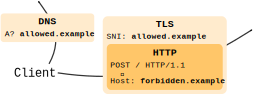
\includegraphics[width=\linewidth]{fronting}
\caption{
Domain fronting uses different domain names at different layers.
At the plaintext layers visible to the censor---the DNS request and the
TLS Server Name Indication---appears
the front domain \mbox{\textbf{allowed.example}}.
At the HTTP layer, unreadable to the censor,
is the actual destination \mbox{\textbf{forbidden.example}}.
}
\label{fig:fronting}
\end{figure}

The censor may block neither the DNS request nor the SNI without
collaterally blocking the front domain.
The Host header is invisible to the censor,
but visible to the server receiving the HTTPS request,
which uses the header to internally route the request to its destination.
No traffic ever reaches the front domain,
which may be oblivious to the circumvention.
For those familiar with decoy routing~\cite{decoyrouting,telex,cirripede,tapdance},
domain fronting can be understood as
``decoy routing at the application layer.''
A fuller comparison with decoy routing appears in Section~\ref{sec:related-work}.

This Wget command shows domain fronting in action
on Google's infrastructure.
Here, an HTTPS request for \urll{www.google.com} has a Host header for
\urll{maps.google.com}. The HTML in the response is that of Google Maps.

\noindent
\begin{quote}
\usefont{U}{cmtt}{m}{n}%
\$ wget -q -O - https://www.google.com/ \char`\\\\
\strut~~~~--header \textquotesingle{}Host: maps.google.com\textquotesingle{} | \char`\\\\
\strut~~~~grep -o \textquotesingle{}<title>.*</title>\textquotesingle{}\\
<title>Google Maps</title>
\end{quote}

Domain fronting works with CDNs because a CDN's frontend server
(called an ``edge server''),
on receiving a request for a resource not already cached,
forwards the request to the domain found in the Host header
(the ``origin server'').
(There are other ways for CDNs to work, but this ``origin pull''
configuration is common.)
% The certificate you get may be that of the front domain,
% or may be a generic shared domain.~\cite{httpsincdn}
Fronting works with Google because Google App Engine, a web application platform,
can host a simple ``reflector'' application that emulates
an origin-pull CDN, simply forwarding every request to another server.
In both cases, the intermediate web service does not forward requests to just anywhere---it
has to be to the domain of a customer.
In order to run a fronting backend,
one generally has to create an account with the web service and pay for bandwidth.

A variation on fronting is ``domainless'' fronting,
in which there is no DNS request and no SNI.
It looks to the censor
like the user is browsing an HTTPS site by its IP address,
or using a web client that doesn't support SNI.
Domainless fronting can be useful when there is no known front domain
with sufficiently high collateral damage.
The censor is faced with the choice of blocking an entire IP address, not only a domain;
blocking requests without SNI;
or trying to find some other, presumably more expensive, test to distinguish
circumvention traffic.

We have developed domain fronting into a full-fledged circumvention system called \meek,
implemented as pluggable transport~\cite{pt} for Tor.
\meek\ combines fronting with an HTTP-based tunneling proxy:
upstream data are transformed into a sequence of HTTP requests,
which are fronted in order to reach a proxy server.
The server decodes the requests and feeds their payloads
into the Tor network.
Downstream data received by the server from Tor
are returned to the client within HTTP responses.
\meek's architecture appears in Figure~\ref{fig:architecture}.
Section~\ref{sec:architecture} describes how it works in detail.

\begin{figure*}
\centering
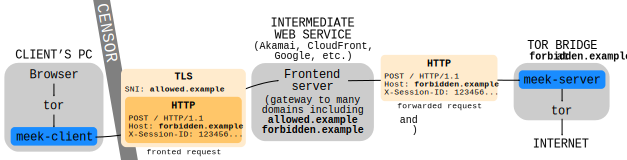
\includegraphics[width=\linewidth]{architecture}
\caption{
Architecture of \meek.
The client sends an HTTP request to the Tor bridge by way of an intermediate web service such as a CDN.
The client protects the bridge's domain name \textbf{forbidden.example} from the censor
by fronting it with another name, here \textbf{allowed.example}.
The intermediate web server decrypts the TLS layer and forwards the request to the bridge
according to the Host header.
The bridge sends data back to the client in the HTTP response.
\meekclient and \meekserver are transport plugins, the interface between Tor and \meek.
The host actually at allowed.example does not participate in the communication.
}
\label{fig:architecture}
\end{figure*}

\meek\ has been built into an experimental release of Tor Browser,
and has a small number of users.
Our deployment so far uses Google App Engine and Amazon CloudFront
as intermediate web service backends.
% with the hidden actual domain \urll{meek-reflect.appspot.com}
% hidden by the front \urll{www.google.com}.
Section~\ref{sec:survey} names other fronting-capable services
and Section~\ref{sec:discussion} describes other possible deployments.
In addition to the Tor pluggable transport,
systems based on \meek\ are now used by other circumvention systems including
[blinded for anonymous submission].
% ANON
% including Psiphon~\cite{psiphon} and Lantern~\cite{lantern}.

% \meek\ is designed to have features attractive in a circumvention transport.
% It is easy to use, not requiring the configuration of any bridge addresses.
% In Tor Browser, users need only select ``meek''
% from a pulldown menu in order to use it.
% It resists blocking by address and by content,
% Section~\ref{sec:discussion}

Domain fronting and HTTPS take care of two big circumvention challenges,
those of hiding the destination and of obscuring the contents of a message.
There remain other, more subtle, attributes of communication
that could serve as a basis for blocking.
For example, the plaintext handshake is a fingerprintable part of TLS.
Section~\ref{sec:browserextension} describes how we use a web browser extension as an instrument for making HTTPS requests,
to make \meek's TLS and HTTPS characteristics
match those of a browser as closely as possible.
Our goal is to force the censor
to employ more sophisticated, expensive, and error-prone statistical tests
to classify traffic as allowed or prohibited,
rather than domain blacklists or deep packet inspection---to
force the practice of censorship to exist in a world
not of simple packet filters,
but of probabilities and false positives.
A preliminary analysis of \meek's resistance to traffic analysis
appears in Section~\ref{sec:trafficanalysis}.
The analysis is based on comparing traffic traces of \meek\
to samples of HTTPS traffic at a network router.

To our knowledge,
the earliest application of domain fronting to circumvention
was by GoAgent~\cite{goagent},
a tool based on App Engine and
once widely used in China.
Fronting has also been used with success since 2013
for the rendezvous component of another transport called flash proxy~\cite{flashproxy}.
GoAgent and flash proxy are the systems that most directly
inspire ours.

% We measure the performance...

\section{Background and related work}
\label{sec:related-work}

Broadly speaking, there are two main challenges in circumvention:
blocking by content and blocking by address.
Blocking by content is based on \emph{what you say},
and blocking by address is based on \emph{whom you talk to}.
A content-blocking censor inspects packets and payloads,
looking, for example, for forbidden protocols or keywords.
Content-based blocking is sometimes called deep packet inspection (DPI).
An address-blocking censor forbids all communication with certain
addresses, for example IP addresses and domain names, whatever the contents of the communication may be.
A savvy censor will use both means of censorship, and
effective circumvention requires countering both.

To the above challenges we add a related one, active probing.
An active-probing censor does not merely passively observe traffic:
it injects its own traffic,
acting as if it were an ordinary client and connecting to suspected
proxy servers to see how they respond.
Then a connection is successful, the server can be blacklisted.
Active probing is a precise means of identifying whether a server belongs to a circumvention system,
even when a protocol is hard to detect on the wire.
Winter and Lindskog~\cite{foci12-winter} confirmed an earlier discovery of
Wilde~\cite{wilde} that China's Great Firewall identifies Tor bridges
by issuing scans that follow up on observed client connections, to discover
whether a server speaks the Tor protocol.
The discovery of active probing was the motivation for probing resistance in ScrambleSuit~\cite{scramblesuit}
and obfs4~\cite{obfs4},
described in this section.


There are two general strategies for countering content-based blocking.
The first is to make traffic look unlike
anything forbidden by the censor; that is, fail to match a blacklist. The second is
to resemble a protocol that is explicitly allowed by the censor; that is, match a whitelist.
Following the first strategy are the so-called ``look-like-nothing'' transports whose
payloads are indistinguishable from a uniformly random byte stream.
Good examples of look-like-nothing transports are
obfs2~\cite{obfs2} and its successor obfs3~\cite{obfs3},
Tor's go-to pluggable transports since early 2012~\cite{obfsproxy-arms-race}.
Both obfs2 and obfs3 work by superenciphering an underlying stream,
using a key exchange that has no plaintext components.
ScrambleSuit~\cite{scramblesuit} is like obfs3 in its
payload obfuscation, but additionally obscures its traffic signature
(packet lengths and timing), and is designed to resist active probing.
A ScrambleSuit server will accept a TCP connection but not send a reply
until the client proves knowledge of a shared secret.
obfs4~\cite{obfs4}
(which despite the name has more in common with ScrambleSuit than with obfs2 and obfs3)
builds on ScrambleSuit with more efficient cryptography and an authenticated handshake.

The other strategy against DPI is the steganographic one: look like
something the censor does not block.
fteproxy~\cite{fte} uses format-transforming encryption to encode data into strings
that match a given regular expression,
for example a regular-expression approximation of HTTP.
StegoTorus~\cite{stegotorus}
transforms traffic to look like a cover protocol
using a variety of special-purpose encoders.
Code Talker
Tunnel (formerly called SkypeMorph)~\cite{skypemorph} mimics a Skype video call.
FreeWave~\cite{freewave} encodes a stream as an acoustic signal
and sends it over VoIP to a proxy.
Dust~\cite{dust} uses encryption to hide static byte patterns and then
shapes statistical features such as packet lengths and byte frequencies so that they
match given distributions.

Houmansadr et~al.~\cite{parrot} evaluate ``parrot'' systems that imitate another protocol
and conclude that unobservability by imitation is fundamentally flawed.
To fully mimic a complex and sometimes proprietary protocol like Skype
is difficult,
because the system must imitate not only the normal operation of the protocol,
but also its reaction to errors,
its typical traffic patterns, and quirks of implementations.
Geddes et~al.~\cite{acks}
demonstrate that even non-parrot systems may be vulnerable to
attacks that disrupt circumvention while having little effect
on ordinary traffic.
Their examination includes VoIP protocols,
in which packet loss and duplication are acceptable.
The censor may, for example, strategically drop certain packets
in order to disrupt a covert channel, without much harming ordinary VoIP calls.


The other grand challenge of proxy-based circumvention is address-based blocking.
Tor has long faced the problem of the blocking of its relays,
the addresses of which appear in a public directory.
In response, Tor began to reserve a portion of its
new relays as secret ``bridges''~\cite{tor-blocking}
whose addresses are not publicly known.
BridgeDB, the database of secret bridges,
carefully distributes bridge addresses
so that anyone can learn a few bridges, but it is hard to learn all of them.
BridgeDB uses captchas and other rate-limiting measures,
and over short time periods,
always returns the same set of bridges to the same requester,
preventing enumeration by simple repeated queries.
BridgeDB is also capable of distributing the addresses
of obfuscated bridges (obfs3 or ScrambleSuit);
the combination
of careful bridge address distribution and obfuscated protocols
gives Tor's system a realistic claim to addressing both main challenges of circumvention.
Address distribution appears to be the weaker side of the defense,
as evidenced by real-world censors' apparent preference for
blocking bridge addresses over real-time DPI-based blocking~\cite{foci12-winter}.

CensorSpoofer~\cite{censorspoofer}
decouples upstream and downstream data channels.
The client sends data to a CensorSpoofer proxy over a low-bandwidth covert channel such as email.
The proxy sends data back over a UDP channel, all the time
spoofing its source address so the packets appear to originate from some other ``dummy'' host.
The censor has no IP address to block, because the proxy's true address never appears on the wire.
Client and server have the challenge of agreeing on a dependable covert upstream channel
that must remain unblocked,
and the client must carry on a believable UDP conversation with the dummy host---a
VoIP call, for example.

Flash proxy~\cite{flashproxy} resists address blocking by
conscripting web users as temporary proxies.
Each JavaScript-based proxy lasts only as long as a
user stays on a web page, so the pool of proxies is constantly changing.
If one of them is blocked, there is soon another to replace it.
Flash proxy's approach to address blocking is in a sense
the opposite of \meek's:
where flash proxy uses many cheap, disposable, individually blockable proxies,
\meek\ uses just a few high-value front domains on hard-to-block network infrastructure.
A quirk of the browser proxy model is that
the client must be able to receive a TCP connection; in particular it
must not be behind network address translation~(NAT), which limits flash proxy's usefulness.
Part of the flash proxy protocol requires the client to send
a small amount of unblockable data in a process called rendezvous.
The default rendezvous mechanism has used domain fronting through App Engine since 2013~\cite{flashproxy-reg-appspot}.
Flash proxy itself does nothing to defend against DPI.
Connections between censored clients and browser-based proxies use
WebSocket, a meta-protocol running on HTTP,
but inside the WebSocket framing is the ordinary Tor protocol.
% There exists a prototype transport that attempts to get both
% content-based and address-based blocking resistance by obfuscating traffic
% with obfsproxy before sending it through flash proxy~\cite{obfs-flash}.
% However it is limited because it is not
% possible to obfuscate the outermost WebSocket layer;
% the censor could decide simply to block all WebSocket.

A technique known as OSS~\cite{oss} (for
``online scanning service'') bounces messages
through web services that are capable of making HTTP requests.
For example, a censored client may ask an HTTPS-based online translation service to
translate the web page at \urll{http://forbidden.example/}\textsl{data...},
where ``\textsl{data...}'' is the URL-embedded message the client wants to send.
The translation service requests the URL,
unwittingly sending the message on behalf of the client.
OSS shares certain similarities with domain fronting:
an unblockable web service takes the place of the front domain,
and the destination of the communication is embedded somewhere in an HTTPS query
rather than in the Host header.

Decoy routing~\cite{decoyrouting}
is a technique that puts
proxies in the middle of network paths, rather than at the ends.
For this reason, it is also called end-to-middle proxying.
Realizations of decoy routing include Telex~\cite{telex},
Cirripede~\cite{cirripede}, and TapDance~\cite{tapdance}.
Decoy routing asks friendly ISPs to deploy special routers that lie
on network paths between censored users and uncensored ``decoy'' Internet destinations.
Circumvention traffic is ``tagged'' in a way that is detectable only
by the special routers, and not by the censor.
On receiving a tagged communication, the router shunts it away from its apparent, \emph{overt destination}
and toward a censored, \emph{covert destination}.
Domain fronting is similar in spirit to decoy routing:
think of domain fronting as decoy routing at the application layer.
In place of a router, domain fronting has a frontend server;
in place of the overt destination is the front domain.
Both systems tag flows in a way that is invisible to the censor:
decoy routing uses, for example, a hash embedded in a client nonce,
while fronting uses the HTTP Host header, encrypted within HTTPS.
Fronting has the advantage that it doesn't require knowing cooperation by network intermediaries.

Schuhard et~al.~\cite{ccs2012-decoys}
introduce the idea of a \emph{routing adversary} against decoy routing,
and show that the connectivity of the Internet enables
censors to force network users onto paths that do not include participating routers.
Simulations by Houmansadr et~al.~\cite{nodirectionhome}
show that even though such alternate paths exist,
they are many times more costly to the censor,
especially when participating routers are placed strategically.

CloudTransport~\cite{cloudtransport} uses cloud storage, for example Amazon~S3,
as a communication channel by encoding sends and receives as reads and writes to shared remote files.
CloudTransport has much in common with domain fronting:
it hides the true endpoint of a communication with HTTPS,
and sends traffic through a domain with high collateral damage.
In CloudTransport, the hidden destination, which is a storage bucket name rather than a domain,
is hidden in the path component of a URL.
For example, in the S3 URL
\urll{https://s3.amazonaws.com/bucketname/filename},
the censor only gets to ``see'' the generic domain part, ``\urll{s3.amazonaws.com}''.
The path component ``\urll{/bucketname/filename}'',
which would reveal the use of CloudTransport,
cannot be used for blocking because it is encrypted inside HTTPS.

GoAgent~\cite{goagent} is a direct inspiration for \meek\ in its use of
domain fronting with App Engine.
Traffic is fronted by the Google frontend server,
using the ``domainless'' fronting model without SNI,
and delivered to its destination by a specialized app running on App Engine.
GoAgent doesn't use an additional general-purpose proxy after fronting;
rather, HTTP and HTTPS URLs are fetched directly from the App Engine servers.
Because of that, GoAgent is limited to carrying HTTP and HTTPS traffic only,
and the contents of all communications are revealed to Google.
Users of GoAgent generally upload their own personal copy of the proxy code to App Engine,
which is free of charge to use as long as they do not exceed a bandwidth quota.
According to a May 2013 survey~\cite{collateral-freedom},
GoAgent was the circumvention tool most used in
China, with 35\% of survey respondents having used it in the previous month.
This figure is higher than that of paid~(29\%) and free VPNs~(18\%), and far
above that of other special-purpose tools like Tor~(2.9\%) and Psiphon~(2.5\%).
Use of GoAgent in China was disrupted starting in the beginning of June~2014
when all Google services (including GoAgent's front domains) were blocked~\cite{cn-google-block}.
\meek\ over App Engine was similarly affected.
% Users identified reliability, speed, and ease of installation as the most important features of a circumvention tool.

Cloud-Entry~\cite{cloud-entry} is somewhat similar to GoAgent.
It also uses App Engine, but uses a socket API rather than a URL fetch API,
in order to support protocols other than HTTP and HTTPS.
Cloud-Entry has the same problem with NAT that flash proxy does,
because the proxy tries to connect back to the client with a socket.
App Engine kills web requests (and their associated socket connections)
when they take longer than 60~seconds,
so users must reconnect at least that often.

Psiphon~\cite{psiphon} is a network of many one-hop proxies,
with encryption and traffic obfuscation between client and server.
% ANON
% Psiphon uses domain fronting based on \meek\ as one of its blocking defenses since June~2014~\cite{psiphon-meek-merge}.
Lantern~\cite{lantern} uses a network of proxies running on volunteer computers;
proxy addresses are shared only with trusted friends in order to make them difficult to enumerate.
% ANON
% Lantern~1.4 is planned to use domain fronting inspired by \meek~\cite{lantern-1.3.1}.

% Infranet
% Freegate
% Ultrasurf

% CORDON? Say how \meek\ would be classified in it?

% Section~\ref{sec:browserextension}, JumpBox
% http://securecomm.org/2014/show/tutorials

\section{Threat model}

The model includes four actors:
the censor,
the censored client,
the intermediate web service,
and the destination Tor bridge.
Circumvention is achieved when the client evades the censor to reach
the bridge,
because the bridge can then proxy to anywhere.
The client and bridge cooperate with each other.
The intermediate web service does not need to cooperate with either,
except to the extent that it doesn't collude with the censor.
% The censor's goal is to prevent circumvention.

The censor controls a network and the links into and within it.
The censor is able to inspect traffic flowing across all links under its control
and may block or allow any packet.
The censor may inject and replay traffic, and
operate its own clients and servers.
The client lies within the censor's network,
while the intermediate web service and bridge lie outside.
The censor blocks direct communication between the client and the bridge,
but allows HTTPS between the client and at least one front domain or IP address
on the intermediate web service.
% In examples, we will use the \textbf{allowed.example} as the front domain
% and \textbf{forbidden.example} as the domain name of the Tor bridge.

% The censor must operate at line rate; that is,
% it must not delay traffic unduly while deciding whether to allow it.
% This consideration is one facet of the censor's sensitivity to
% collateral damage caused by false positives:
% mistakenly blocking or degrading non-circumvention traffic causes the censor
% to incur some penalty, just as mistakenly allowing circumvention traffic does.

The client,
intermediate web service,
and destination proxy
are uncontrolled by the censor.
The censor does not control a TLS certificate authority;
specifically it cannot man-in-the-middle an HTTPS session
without being caught by ordinary certificate verification.
The client has a way to get a copy of the necessary client programs.

Section~\ref{sec:discussion} shows what happens when some
of the threat model's assumptions are violated;
specifically what happens
when the intermediate web service's frontend server is inside the censor's network
and when the censor controls a certificate authority.

\section{Architecture and protocol of meek}
\label{sec:architecture}

The components of the system are shown in Figure~\ref{fig:architecture}.
The parts that are new in \meek\
are the programs \meekclient and \meekserver,
which are \meek's interface with Tor.

\meekclient is essentially a web client that knows how to front HTTPS requests.
When \meekclient receives an outgoing chunk of data from a client Tor process, it bundles it up into a POST request
and fronts the request through the web service,
which in turn forwards it to \meekserver on the bridge.
If the response returned by \meekserver contains any HTTP body,
\meekclient decodes the body and sends it back to the Tor client.
\meekclient takes pains to make its TLS fingerprint
look like that of a browser; see Section~\ref{sec:browserextension}.

\meekserver is a special-purpose web server.
When \meekserver receives a request, it extracts the body and feeds it into
the Tor network.
If there is anything pending to be sent back to the client from Tor,
\meekserver includes it in the body of the HTTP response.
\meekserver also handles session management:
keeping track of which requests correspond to which active Tor connection.

When \meek\ is used with Google App Engine, one other component is needed:
a small ``reflector'' web app that simply copies any request
it receives and forwards it to a remote instance of \meekserver.
App Engine cannot directly run a Tor bridge,
so we bounce the requests to somewhere that can.
The reflector app emulates the behavior of an origin-pull CDN,
which also simply copies and forwards requests
when the response is not already cached.

The main technical challenge of the protocol is splitting a TCP stream up
into a sequence of HTTP requests and responses.
The body of each HTTP request and HTTP response carries
a small chunk of upstream or downstream communication.
There must therefore be some way of making sure that chunks
are correctly reassembled at the other end,
in order and without gaps or duplicates.
\meek\ takes a naive approach: requests and responses are strictly serialized.
The client doesn't send a second chunk of data
(i.e, make another HTTPS request) until it has
received the response to its first.
The reconstructed stream is simply the concatenation
of bodies in the order they arrive.
Handling stream reconstruction this way is simple and guarantees correctness,
but has performance drawbacks because there is a full round-trip
between every send.
Section~\ref{sec:discussion} proposes a more efficient encoding
that would enable multiple requests in parallel.

\begin{figure}
\scriptsize
\begin{verbatim}
POST / HTTP/1.1
Host: forbidden.example
X-Session-Id: cbIzfhx1Hn+RHURmIPhjgY+W3B6zA8Ua6dd92DLscOE=
Content-Length: 517

\x16\x03\x01\x02\x00\x01\x00\x01\xfc\x03\x03\x9b\xa9...
\end{verbatim}
\begin{quote}
\begin{verbatim}
HTTP/1.1 200 OK
Content-Length: 739

\x16\x03\x03\x00\x3e\x02\x00\x00\x3a\x03\x03\x53\x75...
\end{verbatim}
\end{quote}
\begin{verbatim}
POST / HTTP/1.1
Host: forbidden.example
X-Session-Id: cbIzfhx1Hn+RHURmIPhjgY+W3B6zA8Ua6dd92DLscOE=
Content-Length: 0

\end{verbatim}
\begin{quote}
\begin{verbatim}
HTTP/1.1 200 OK
Content-Length: 75

\x14\x03\x03\x00\x01\x01\x16\x03\x03\x00\x40\x06\x84...
\end{verbatim}
\end{quote}
\caption{
Requests and responses in the \meek\ HTTP protocol.
The session ID is randomly generated by the client.
Request/response bodies contain successive chunks of a Tor TLS stream
(\texttt{\textbackslash{}x16\textbackslash{}x03\textbackslash{}x01\textbackslash{}x02}
is the beginning of a TLS ClientHello message).
The second POST request is an empty polling request.
The messages shown here is encrypted inside HTTPS until after
it has been fronted,
so the censor cannot use the
Host and \mbox{X-Session-Id} headers for classification.
}
\label{fig:protocol}
\end{figure}

\meekserver must handle many clients at once,
and therefore maintains many open connections to a local Tor process,
one for each active client.
When a new request arrives, the server must determine which
open session it belongs to
(or whether it is a brand-new client needing a new session).
In TCP, different streams are distinguished by their
(source~IP, source port, dest~IP, dest~port) tuple,
but that doesn't work for \meek, for two reasons:
the source IP of the requests is that of the intermediate web service,
not of the actual client;
and a logical stream is chopped into multiple independent HTTP requests,
so the source port is always changing.
Instead, each client generates a random 256-bit session ID for each new Tor stream,
which it sends with its requests in a special
\mbox{X-Session-Id} HTTP header.
\meekserver, when it sees a session ID for the first time,
opens up a new connection to the local Tor process
and associates the connection and ID in a cache.
Subsequent requests with the
same session ID will reuse the same Tor connection.
Sessions are closed after a period of inactivity.
Figure~\ref{fig:protocol} shows a sample of the protocol.

HTTP is fundamentally a request-based protocol.
There is no way for the server to ``push'' data to the client without
having first received a request.
In order to enable the server to send back data,
\meek\ uses one of two techniques.
The first is polling:
every so often the client sends a request with an empty payload
if it has nothing else to send,
simply to give the server an opportunity to send something back.
The polling interval starts short (100~ms) and grows exponentially
up to a maximum of 5~s.
% ANON
% The other technique,
% implemented in Psiphon's version of \meek,
The other technique
uses streaming HTTP responses over persistent HTTP connections.
When the server sends a response, it keeps the connection open,
continually appending data to the response body while it has anything to send.
When the server receives a new request from the same client,
it closes any response stream it has open to that client and starts a new one.
This second technique is especially beneficial for bulk downloads,
but doesn't work on all services:
notably Google App Engine doesn't support streaming of this kind.

As an encrypted tunneling protocol, meek necessarily adds overhead.
Each chunk of data gets an HTTP header, and then the HTTP
request is wrapped in TLS.
We estimate the overhead when meek is used to transport Tor.
Tor uses fixed-size cells of 514 bytes~\cite[Section~0.2]{tor-spec}.
Each cell is wrapped in a TLS Application Data record, which adds 29 bytes
when using a GCM ciphersuite (the default in current versions of Tor).
% (in Tor version~0.2.4.22 using a GCM ciphersuite).
This 543-byte record is received by \meekclient,
which adds an HTTP header whose length is about 400 bytes
(varying slightly depending on the length of the Host field).
The HTTP request goes into its own TLS Application Data record when it becomes HTTPS,
adding about 50~bytes
depending on how much padding is used by the ciphersuite in use.

% 514 → 543 → 956 → 1013

\begin{center}
\begin{tabular}{r@{}r l}
          &    514 & Tor cell \\
          &  $+$29 & Tor TLS record \\
$\approx$ & $+$400 & \meek\ HTTP header \\
$\approx$ &  $+$50 & \meek\ TLS record \\
\hline
$\approx$ &   1000 & total
\end{tabular}
\end{center}

% >>> (1*543+450.)/(1*543)
% 1.828729281767956
% >>> (2*543+450.)/(2*543)
% 1.4143646408839778
% >>> (3*543+450.)/(3*543)
% 1.276243093922652
\noindent
The total overhead varies according to the length
of the Host field in the header and the specifics of the intermediate web service's TLS configuration,
but is somewhere in the neighborhood of $(543+450)/543-1\approx83$\%.
This is the worst case, when Tor sends a single cell.
Tor can bunch multiple cells into one transmission;
if two cells are sent at once, the overhead drops to
${\approx}41$\%; if three, it is ${\approx}28$\%.
Bulk uploads and downloads tend to have less overhead, bunching many cells at once.
Streaming HTTP responses, when they are possible, reduce overhead further,
% ANON
% Persistent HTTP connections as used by Psiphon reduce overhead further,
because only one HTTP header is needed for a large number of transmissions.
Empty polling requests also use bandwidth,
but they are sent only when the connection is idle,
so they don't affect upload or download speed.
As is discussed in Section~\ref{sec:trafficanalysis},
\meekclient reuses the same TLS connection for many requests,
so the fixed overhead of the initial TLS handshake is amortized.

% Mention server--client overhead?
% The same except for HTTP header.

There is additional latency overhead caused by meek's extra network hop:
rather than accessing the Tor bridge directly,
the client first goes to the intermediate web service.
How much latency the extra hop adds depends, of course, on the network location
of the client, web service, and Tor bridge.
Strict serialization of requests and responses
becomes a problem with large round-trip times,
as throughput becomes limited by latency.
Section~\ref{sec:discussion} describes ways to improve
performance with high latencies.
% ANON
% performance with high latencies;
% Psiphon's use of persistent connections as described in this section is one of them.

\section{Camouflage for the TLS layer}
\label{sec:browserextension}

Domain fronting defeats address-based blocking and active probing.
HTTPS foils simple DPI,
hiding any byte patterns in the underlying stream.
The censor may also apply DPI to the tunnel itself in order to try to
distinguish fronted from non-fronted traffic.
This section is about TLS fingerprinting,
which is the censor's remaining easy distinguisher,
and how we use a web browser with an unremarkable TLS fingerprint
to disguise the HTTPS tunnel.
Section~\ref{sec:trafficanalysis} is about more subtle and hard-to-apply forms of traffic analysis.

The TLS handshake is largely plaintext~\cite[Section~7.4]{rfc5246}, and leaves
enough room for variation, for example in
the client's lists of ciphersuites and extensions,
that it is possible to fingerprint different client TLS implementations~\cite{ssl-p0f}
based on their handshake.
(We are only concerned with fingerprinting the client,
because the server's TLS
comes from the intermediate web service;
i.e., it is what you would expect to see when connecting to the front domain.)
Tor itself was blocked by China in 2011
because of the distinctive ciphersuite list it used at that time~\cite{bug4744}.
Figure~\ref{fig:ciphersuites} in Appendix~\ref{sec:ciphersuites} shows examples of how TLS client
implementations may detectably differ.
\meekclient is written in the Go programming language,
which has a custom TLS library~\cite{golang-crypto/tls};
Figure~\ref{fig:ciphersuites:golang}
shows how it would appear on the network with no TLS camouflage.
Figures~\ref{fig:ciphersuites:firefox} and~\ref{fig:ciphersuites:chrome}
show two browsers which have TLS fingerprints different from Go's
and different from each other's.
A censor could block an uncamouflaged \meek\ using Go's TLS fingerprint,
if it considered the collateral damage resulting from blocking other Go programs to be slight enough.

In order to disguise its TLS fingerprint,
\meekclient proxies all its HTTPS requests through an actual web browser.
We implemented extensions for two web browsers,
Firefox and Chrome,
that enable them to make HTTPS requests on behalf of \meekclient.
The TLS fingerprint looks like that of a browser, because it is that of a browser.
The browser instance running the extension is completely separate
from the browser the user interacts with.
It runs invisibly in the background in a separate process,
doesn't display a user interface,
and shares no state with the user's browser.

\begin{figure}
\centering
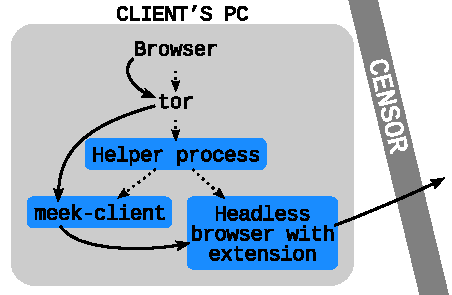
\includegraphics[height=1.5in]{browser-architecture}
\caption{
Client architecture including a browser extension for TLS camouflage.
Dashed lines show the process hierarchy.
Solid lines show the flow of outgoing communication.
The headless browser runs in the background and is invisible to the user.
This figure is a zoomed-in view of the ``Client's PC'' component of Figure~\ref{fig:architecture}.
}
\label{fig:browser-architecture}
\end{figure}

Figure~\ref{fig:browser-architecture} shows the interaction of components
on the client's computer.
The local Tor process runs a helper process that starts both \meekclient
and the headless browser,
then configures \meekclient to proxy its requests through the browser extension.
The user's browser proxies through Tor;
Tor proxies through \meekclient;
and \meekclient proxies through the headless browser.
The headless browser is the only part that ever actually touches the network.
It should be emphasized that the URLs requested by the headless browser extension
have no relation to the URLs the user browses;
the extension only ever makes requests to the front domain.

The use of a browser extension brings benefits beyond TLS camouflage.
It means \meek's HTTP tunnel inherits other characteristics of the browser:
for instance
how often it resolves DNS,
its connection reuse,
and its HTTP keepalive behavior.
The Firefox extension has special advantages
when \meek\ is used with Tor Browser
because Tor Browser
is a modified version of Firefox:
we can use the same browser executable for both the browser the user interacts with (Tor Browser)
and the one providing TLS camouflage (headless Firefox),
saving space in distribution packages
and sparing the user the chore of having to separately configure a browser to run the extension.
In Tor Browser,
the headless Firefox is started and stopped transparently
when \meek\ is activated and deactivated.

% The development of the browser extensions posed some unexpected challenges.
% Tor Browser disables TLS session tickets because they can be used as linking identifiers,
% but the lack of session tickets shows up as a missing TLS extension,
% so we had to reenable them in the headless browser.
% (Doing so doesn't harm Tor Browser's anonymity:
% if session tickets are used, they are used only on the circumvention layer
% between the user and the frontend server. Tor Browser's own TLS is tunneled
% within the circumvention layer, and session tickets are still disabled at that level.)
% The Chrome extension needed to be split into two pieces, an extension and an app,
% because an extension cannot open a listening socket and an app cannot make HTTP requests.

No TLS camouflage is needed between the intermediate web service and \meekserver,
because that portion of the communication flow is not observed by the censor.

Appropriate TLS camouflage may differ depending on circumstances.
On a traditional desktop PC, using a browser is probably the right choice.
When
[blinded circumvention tool]
% ANON
% Psiphon
ported \meekclient to Android,
they didn't use a browser as camouflage,
but rather made all HTTPS requests with the standard Android HTTP API.
This decision makes sense because other Android applications
also use the standard API and share the same TLS fingerprint.

\section{A survey of fronting-capable\\web services}
\label{sec:survey}

This section contains a brief survey of fronting-capable
web services we have found, each with its pros and cons.
The list is not exhaustive and is meant to illustrate the broad
support for fronting that exists.
Of the services listed, we have so far deployed \meek\
only on Google App Engine and Amazon CloudFront.
For the others, we have only checked that fronting works.
Recall that even web services that support fronting
will front only for their own customers,
so new each deployment typically requires an investment of time and money.

Google App Engine~\cite{googleappengine}
is a web application platform.
Each application gets a user-specified subdomain of \urll{appspot.com},
which can be fronted through almost any Google domain,
including google.com, gmail.com, googleapis.com, and many others.
App Engine can run only web applications,
not a full Tor bridge;
for that reason we use a tiny ``reflector'' application
that merely copies incoming requests to a Tor bridge hosted elsewhere.
Fronting through App Engine is attractive in the case where
\urll{appspot.com} is blocked---not unlikely,
because of the ease of building a proxy there---but
at least one other Google service is reachable.
Applications that use less than one gigabyte of bandwidth daily
are free of charge,
making possible an upload-your-own-app model
à la GoAgent.

Amazon CloudFront~\cite{cloudfront},
not to be confused with CloudFlare,
is the CDN of Amazon Web Services.
A CloudFront ``distribution'' associates
an automatically generated subdomain of \urll{cloudfront.net}
with an origin server,
which in our case is an instance of \meekserver.
The front domain may be any other of CloudFront's automatically generated subdomains, all
of which support HTTPS through a wildcard certificate.
CloudFront has a usage tier that is free of charge for a year,
subject to a bandwidth limit of 50 gigabytes per month.

Microsoft Azure~\cite{azure}
is a cloud computing platform that features a CDN.
Similarly to CloudFront, users get automatically generated subdomains
of \urll{vo.msecnd.net},
all of which can front for each other.
The CDN works only for Azure domains, however,
so as with App Engine, it is necessary to run a trivial reflector app
that merely forwards requests out of Azure toward an external proxy.
There are other front domain names, like \urll{ajax.aspnetcdn.com},
that may offer high collateral damage.

CloudFlare~\cite{cloudflare},
not to be confused with CloudFront,
is a CDN also marketed as protection against
denial-of-service attacks.
It appears that any domain name on CloudFlare
can front for any other, even custom user-selected domains;
however it is not obvious which one is best to use as a front.
The front domain needs to be a popular one
(causing high collateral damage if blocked),
or the censor may simply block it entirely.
It is doubly bad when a domain is blocked in this way,
because not only is circumvention foiled,
but some unsuspecting third party has just had their web site blocked.
A solution may be to round-robin through
a pool of popular domain names;
or to use ``domainless'' fronting that doesn't send SNI.
% Though CloudFlare supports domain fronting,
% its terms of service~\cite{cloudflare-terms}
% seem to prohibit the kind of tunneled proxying that \meek\ does:
% \begin{quote}
% \textsc{Section 10: Limitation on non-HTML caching}\\
% You acknowledge that CloudFlare's Service is offered as a platform to cache and
% serve web pages and websites and is not offered for other purposes
% \ldots\ you understand and agree to use the Service solely
% for the purpose of hosting and serving web pages\ldots
% \end{quote}

Akamai~\cite{akamai-site} is a large CDN.
Requests may be fronted through the special HTTPS domain
\urll{a248.e.akamai.net},
which serves a certificate also good for \urll{*.akamaihd.net}.
The collateral damage of blocking Akamai is enormous:
in 2010 it carried 15--20\% of all web traffic~\cite{akamai}.
Akamai costs more than other CDNs;
it would likely require institutional support
to keep a circumvention system running on it in the long term.

Fastly~\cite{fastly} is a CDN.
It is the only one of the services we tested in that
that appears to enforce SNI:
if the SNI and Host do not match,
the Fastly edge server returns an HTTP 400 (``Bad Request'') error.
However, if the TLS ClientHello omits SNI, then the Host may be any Fastly domain.
It is the only service we have found
that requires the ``domainless'' fronting style.

\section{Traffic analysis}
\label{sec:trafficanalysis}

One of our goals in developing \meek\ is to force
the censor to use relatively more expensive statistical classifiers
to effect blocking---generally, to increase the cost of censorship.
We believe \meek\ is resistant to the ``easy''
forms of blocking, namely IP address and DNS blocking,
simple pattern-based DPI,
and active probing.
We hope to force the censor to resort to measuring
more subtle features of the communication.
In this section we provide a preliminary analysis
of \meek's resistance to such attacks.
Specifically, we consider three traffic features:
packet length distribution,
number of simultaneous connections,
and connection lifetime.

The issue of statistical traffic analysis is a general one~\cite{trafficmorphing},
and mostly orthogonal to \meek's main idea, domain fronting.
It may be that the problem of traffic analysis is
best solved by a modular component not
necessarily specifically designed for \meek.

% Advantage is that we are probably proxying web traffic.
As \meek\ is based on HTTPS,
we compare traffic traces of \meek\ against
traces of ``ordinary'' HTTPS traffic.
We did a packet capture
of automatically browsing the home pages
of the top 500 Alexa web sites using \meek\ in Tor Browser,
with the browser camouflage described in Section~\ref{sec:browserextension},
and Google App Engine as the intermediate web service.
The \meek\ trace is 687~megabytes in all
and covers about 4.5 hours of network activity.
Our representative of ordinary HTTPS traffic
is a sanitized 10-minute trace
from 
%Lawrence Berkeley National Laboratory (\lbl)
a research lab [blinded as \lbl for anonymous submission],
comprising data to and from TCP port 443 on any Google server.
% Mention the non-google if it appears in a figure.
The \lbl trace consists 313~megabytes of packet headers,
not payloads, destined for TCP port 443 on any Google server.
The original IP addresses were masked by being
replaced by a counter before we received the trace.

\begin{figure}
\centering
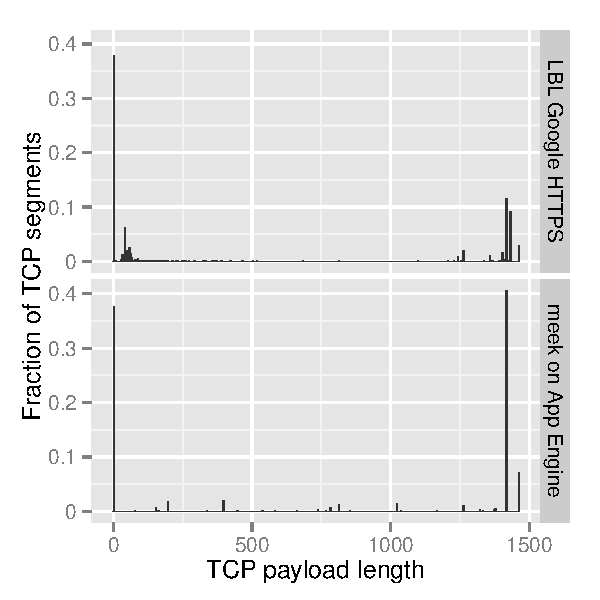
\includegraphics[width=\linewidth]{datalen.pdf}
% Output of datalen.R.
%
% LBL
%          0       1430       1418         41       1416       1460       1260
% 0.37665361 0.09120402 0.08493944 0.06090732 0.03101247 0.02941974 0.02021770
%       1400       1359         33
% 0.01673740 0.01126137 0.01100281
%
% meek
%        1418           0        1460         396         196        1024
% 0.405280243 0.376703906 0.071561089 0.019905460 0.018484996 0.014868083
%         811         783         151        1263
% 0.012312668 0.007811963 0.007031241 0.006569205
\begin{tabular}{r r >{\qquad} r r}
\multicolumn{2}{c}{\lbl Google HTTPS} & \multicolumn{2}{>{\qquad}c}{\meek\ on App Engine} \\
0 bytes & 37.6\% & 1418 bytes & 40.5\% \\
1430 bytes & 9.1\% & 0 bytes & 37.7\% \\
1418 bytes & 8.5\% & 1460 bytes & 7.2\% \\
41 bytes & 6.1\% & 396 bytes & 2.0\% \\
1416 bytes & 3.1\% & 196 bytes & 1.8\% \\
1460 bytes & 2.9\% & 1024 bytes & 1.5\%
\end{tabular}
\caption{
Comparison of TCP payload length distributions
between ordinary HTTPS connections to Google services
from the \lbl traffic trace,
and \meek\ running on App Engine, fronted through www.google.com.
% The histogram's bin width is 5~bytes.
}
\label{fig:datalen}
\end{figure}

\subsection{Packet lengths}

Protocols vary in their packet lengths;
a censor may block a circumvention protocol if its length distribution
is distinct enough.
Figure~\ref{fig:datalen}
compares the packet length distributions of the sample traffic traces.
In both cases, about 38\% of packets have an empty payload, mostly ACKs.
There is a small peak in both traces at the usual TCP Maximum Segment Size
of 1460 bytes.
The concentration of values near 1418 bytes
may be caused by Google servers' sizing of TLS records so they fit within TCP segments.
% https://github.com/joyent/node/issues/6889
% http://mailman.nginx.org/pipermail/nginx-devel/2013-December/004703.html
Conspicuous in the \meek\ trace are a small number of
discrete frequent packet sizes,
and the lack of a cluster of short payloads of around 50 bytes.
Both of these characteristics are probably reflections
of Tor's fixed cell size and the nearly fixed-size HTTP headers
added by \meekclient and \meekserver.
% In this trace, packets of 1024 bytes are probably single
% Tor cells and those of 396 are probably empty polling requests.

% David: I don't think the following paragraph is true.
% Almost all the length>1400 packets are Google→client, not client→Google,
% as you can see if you split the histogram up by direction.
%
% To explain the phenomenon, recall that we use browsers to handle HTTPS connections for \meek\ in order
% to hide TLS handshake characteristics.
% Browsers also apply techniques like HTTP pipelining to improve performance. Since \meek\ is always communicating with
% the same Google frontend server, the browser will keep the persistent TLS connection. In addition, small requests 
% can be batched into a large chunk before being sent. This explains why large packets are mostly seen from the trace that
% records \meek's traffic.
% In contrast, normal users may not have persistent connections to Google. For example, a user may search a keyword on
% Google, click a result, and then close the tab that displays search results. The browser may close the 
% connection immediately after the user leaves the Google web page. Next time the user browses Google search, the browser 
% opens a new connection. In this case, small requests do not have such opportunity for batching.

% These browser techniques improve performance, but also pose unexpected consequences. 
% Although \meek\ alters the packet size distribution of underlying Tor traffic, 
% the censor may be aware of the distribution of \meek\ itself. 
% Additionally, the persistent connection itself can be an issue.
% We thus investigated other related characteristics.

\subsection{Connection lifetime}

\begin{figure}
\centering
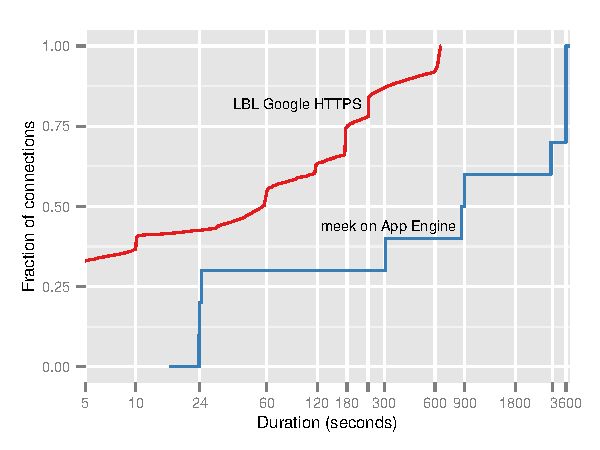
\includegraphics[width=\linewidth]{flowduration}
\caption{
CDF of connection lifetime.
The horizontal axis is logarithmic.
\meek's connections tend to last longer than those of ordinary HTTPS traffic.
}
\label{fig:duration}
\end{figure}

% Output of flowduration.R.
% LBL
% [1] "42.6%" "87.0%" "92.2%"
% meek
% [1] "10.0%" "30.0%" "40.0%"

We consider the duration of TCP connections as a potential distinguisher.
Figure~\ref{fig:duration} shows the cumulative probability
of connection durations in our two traces.
Considering the \lbl trace first,
we see interesting probability concentrations on
round numbers: 10~s, 60~s, 120~s, 180~s, and 240~s.
We hypothesize that this phenomenon is caused by
keepalive timeouts in web browsers and servers,
and polling behavior of web apps.
The small rise at 600 seconds is an artifact caused
by the fact that the trace is only 10 minutes long.
Connections lasting longer than 10 minutes are not accurately reflected,
however we can say that only about 8\% of connections lasted longer than 10 minutes.

The \meek\ trace shows a propensity for longer connections.
Over 4.5 hours, there were only 10 connections,
three of them lasting for an hour.
The long connections are caused by the client browser extension's
use of long-lived HTTP keepalive connections,
combined with \meekclient's polling requests,
which keep the connection from becoming idle.
The traffic trace represents the browsing of hundreds of web sites
and thousands of HTTPS transactions, but they all
occurred over just a few TCP/TLS connections.
60\% of \meek\ connections lasted five minutes or longer,
while only 13\% of those of ordinary traffic did.
\meek\ has essentially no connections lasting less than 24 seconds,
but such short connections account for over 42\% of the \lbl trace.
30\% (3 out of 10) of \meek's connections lasted almost exactly one hour,
evidently reflecting a built-in time limit in either the client browser extension
or in App Engine.

In light of these findings,
the censor may decide to block any long-lived HTTPS connections between
a client and a web service.
According to our traffic trace, doing so will not disrupt more than 8\% of ordinary connections;
whether that is an acceptable cost depends on the time threshold and the censor's
tolerance for collateral damage.
The censor can lower the timing threshold, at the cost of more false positives.
Duration-based blocking is favorable for the circumventor,
because if the censor terminates connections after, say, 10 minutes,
in any case that's 10 minutes of circumvention achieved,
after which \meek\ can start a new connection
and allow Tor to rebuild its circuits.
Future enhancements in \meek\ may even allow reconnecting using the same session ID,
so there will be no effect on the client other than a brief delay
while a new HTTPS connection is established.

% meek is fairly robust against connection termination.
% Well, not really for long-lived TCP connections.
% But it could be.
% Can reconnect and make a new circuit.

\subsection{Concurrent connections}

% Output of concurrent.R.
% [1] 2745
% [1] 2.610621
% [1] 1
% [1] 1.002148
% [1] 772
% [1] 2745
% [1] 0.2812386

\begin{figure}
\centering
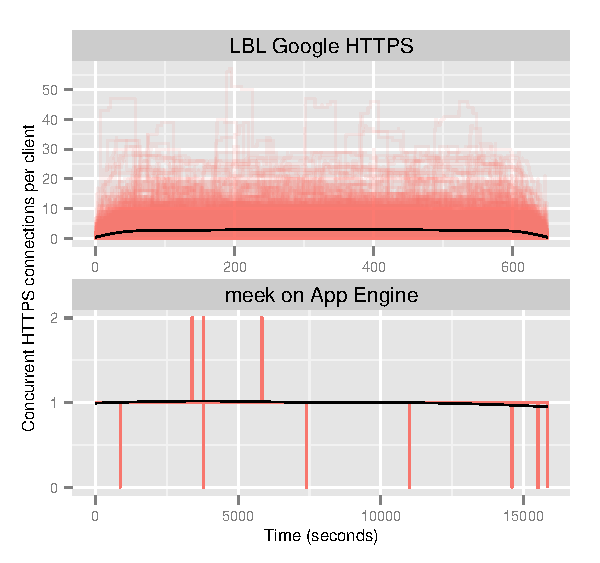
\includegraphics[width=\linewidth]{concurrent.pdf}
\caption{
Number of simultaneous HTTPS connections to any Google server.
Each pale line indicates the number of HTTPS connections
of a single client IP address.
The \lbl trace shows 2,745 unique clients and the \meek\ trace only one.
The dark line is a smoothed average number of connections per client.
The \meek\ count stays close to~1 throughout, only momentarily
jumping to 0 or~2.
The average number of connections per user in the \lbl trace is 2.61,
and in the \meek\ trace is 1.002.
}
\label{fig:concurrent}
\end{figure}

The number of concurrent connections is another potential distinguisher.
We have seen how \meek\ tends to use one long-lived connection
through which it tunnels all its requests.
Figure~\ref{fig:concurrent} compares the number of concurrent HTTPS connections to
Google per client in both traces.
The number of connections in the \lbl trace is variable,
with some hosts briefly spiking up above 50 connections,
but the average case is very heavily skewed to smaller numbers.
The average number of connections in the \lbl trace is 2.61,
with 28\% of clients never having more than 2 concurrent connections.
In the \meek trace the average is almost exactly 1, only briefly
deviating when one connection ends and another begins.
We conclude that having a small number of concurrent connections is unremarkable.


% $$\diamondsuit$$

So far we do not find any obvious traffic characteristics that can be useful to reliably distinguish \meek\
from other HTTPS traffic.
The long-lived connections and few common packet sizes are
potential targets for a more concerted attack.
The fundamental problem we face is essentially that of steganography,
the need to make our traffic fit some model of ``normal'' traffic.
The problem is inherently difficult,
because it is difficult to say just what normal traffic \emph{is}.
It depends on the network environment;
it also depends on the endpoint.
Google's traffic is different than Akamai's.

For the purposes of censorship circumvention,
one doesn't need to match exactly a ``typical'' traffic profile;
only not to deviate from it too much.
Circumvention traffic must only be difficult enough to distinguish from ordinary traffic
that blocking it requires an amount of false positives unacceptable to the censor.
Even 1\% of Google traffic accidentally blocked may exceed the collateral damage tolerance of some censors.
Further, it is hard to characterize what normal use is of, say, a CDN:
they provide access to ordinary web sites,
but also to video streams and software updates,
and not all clients are web browsers.
The difficulty we face is symmetric;
if finding the right model is difficult task for us,
it is also difficult for the censor.
We have seen that censors prefer to use easy classifiers when they exist.
By removing the easy ways, we increase the censor's cost.

\section{Deployment}
\label{sec:deployment}

Development on \meek\ as a Tor pluggable transport~\cite{pt} began in January~2014.
Our target for deployment is Tor Browser~\cite{torbrowser},
a customized version of Firefox that is
preconfigured to use a built-in Tor client.
% and patched to defend against application-layer privacy and anonymity threats
% like tracking cookies and web browser fingerprinting.
Tor Browser has an easy interface for selecting pluggable transports.
% ANON
% [Some details of deployment are omitted for anonymous submission.]
% We made a series of experimental releases of Tor Browser featuring \meek,
% releasing the first one on February~18.
% On April~18 we made the first release featuring the browser camouflage
% that is the subject of Section~\ref{sec:browserextension}.
% We announced our releases on Tor development mailing lists,
% whence they were picked up by Tor Weekly News on the Tor blog.
% Our code was merged by the Tor Browser maintainers
% in June and is scheduled for an alpha release,
% still pending as of this writing.

We have so far deployed on three backends:
Google App Engine,
Amazon CloudFront,
and Microsoft Azure.
Figure~\ref{fig:clients-tor} shows the daily average number of concurrent users of \meek.
(A measurement of 500, for example, means that there were on average 500
users of the system at any given time during the day.)
The App Engine backend was established in February;
CloudFront in July;
and Azure in October.
Also in Figure~\ref{fig:clients-tor} is a table of monthly costs for each web service.
The pricing for cloud services is complicated,
depending not only on bandwidth but also on geographical region and other factors.
For example CloudFront charges per request as well as per gigabyte,
and about 54\% of the CloudFront bill for October was for requests.
App Engine charges extra when it has to run multiple instances
of an app's code to cope with load;
about 15\% of October's App Engine bill was for such ``instance hours.''
% These and other cost details are summarized in a mailing list post~\cite{meek-costs-201410}.
The App Engine and CloudFront backends are running on accounts
that provide a limited amount of free bandwidth,
but current use greatly exceeds the free thresholds.
Azure service is being donated and so has not yet cost anything.
The total cost so far has been \$187.13,
but this number is expected to more than double in November and continue to increase.

\begin{figure}
\centering
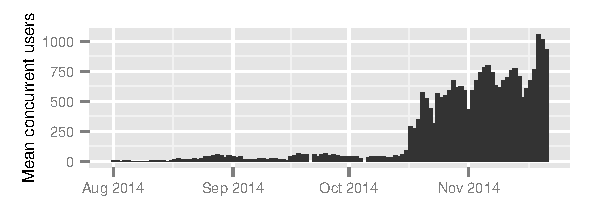
\includegraphics[width=\linewidth]{clients-meek}
\begin{tabular}{l r r r}
       &App Engine &CloudFront&  Azure \\
\hline
Jan--Jul &  \$2.72 &   \$0.00 & \$0.00 \\
Aug      &  \$1.56 &   \$3.10 & \$0.00 \\
Sep      &  \$4.02 &   \$4.59 & \$0.00 \\
Oct      & \$40.85 & \$130.29 & \$0.00 \\
\hline
total    & \$49.15 & \$137.98 & \$0.00 \\
\end{tabular}
\caption{
Concurrent users of the \meek\ pluggable transport
and month-by-month operational costs.
The total cost to date is \$187.13.
% ANON
% The large increase of users on October~15 coincides with
% the release of Tor Browser~4.0,
% the first release to make meek easily available.
Azure CDN service is currently being donated as part of a research grant.
The user estimates come from the Tor Metrics Portal~\cite{metrics-meek,counting-daily-bridge-users}.
}
\label{fig:clients-tor}
\end{figure}

% \begin{figure}
% 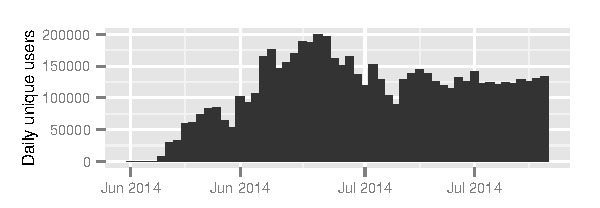
\includegraphics[width=\linewidth]{clients-psiphon3}
% \caption{
% Daily unique users of \meek\ with
% [blinded circumvention tool]
% % ANON
% % Psiphon
% (note vertical axis).
% The decrease at the end of June
% was caused by an unblocking event that made \meek\ unnecessary for some users.
% }
% \label{fig:clients-psiphon3}
% \end{figure}

%  &\$49.15 & \$137.98 & \$0.00 & \$187.13 &  \\

% which aggregates statistics reported by Tor relays.
% The number of users is estimated by counting the number
% of Tor directory requests made by clients~\cite{counting-daily-bridge-users}.

% [Blinded circumvention tool]
% % ANON
% % Psiphon
% began their independent deployment of \meek\ in June~2014.
% Figure~\ref{fig:clients-psiphon3} shows the number
% of unique daily users of \meek%
% ,
% % ANON
% % with Psiphon,
% estimated through clients' self-reporting of their most recent connection date.
% The developers tell us that the drop that occurs
% in the middle of June was not caused by a blocking event,
% but rather an unblocking event that made \meek\ unnecessary for some users.
% Although Figures~\ref{fig:clients-tor} and~\ref{fig:clients-psiphon3}
% are not directly comparable because they count slightly different things,
% it is clear that meek-with-%
% [blinded circumvention tool],
% % ANON
% % Psiphon,
% with its thousands of daily users,
% is much more widely used than meek-with-Tor, which has not yet seen a formal release.

As users increase, it becomes more pressing
to find a way to sustain continued operation.
Although some of the systems listed in Section~\ref{sec:survey}
are inexpensive enough that some users could upload their own fronting backend
and bear their own costs,
we believe that there are compelling usability advantages
to operating a centralized backends for the use of the public.
Client software can ship with preconfigured domain names.
There is nothing for the user to upload and no out-of-band bootstrapping communication is needed.

% The number of parties able to analyze users' traffic patterns is somewhat increased:
% the path from user to Tor bridge now includes App Engine and the web app operators,
% in addition to the ISP and intermediate routers that were there before.
% On the other hand, the Tor bridge no longer gets to see users' IP addresses:
% all it sees are many connections from App Engine.

\section{Discussion}
\label{sec:discussion}

Domain fronting derives its strength from the
high collateral damage of blocking the fronted-through domain.
To front through \urll{www.google.com} to App Engine, for example,
is to make a bet that the censor will lack the temerity to block Google.
Different censors will differ in their aversion to collateral damage;
blocking an important service is a costly measure
that harms users not involved in circumvention and perhaps a society's economic well-being,
and not all censors can afford to do it.
The Great Firewall of China took the unprecendented step
of blocking all Google services in June 2014~\cite{cn-google-block,cn-google-block-greatfire},
and has since blocked certain CDN domains that were used to host
mirrors of censored web sites, even at the cost of damaging other unrelated sites~\cite{cn-edgecast-block-greatfire}.
In 2012, the government of Pakistan blocked all of YouTube
in order to restrict access to one video,
and in 2011, the government of Egypt briefly completely ``turned off the net.''
% http://www.washingtonpost.com/business/economy/youtube-blocked-in-pakistan/2012/09/17/30081fa2-00ea-11e2-b257-e1c2b3548a4a_story.html
% https://en.wikipedia.org/wiki/Internet_censorship_in_Egypt#2011_Internet_shutdown
These examples show that blocking resistance is not an absolute,
black-and-white security property;
it can only be discussed in an economic context, relative to the costs borne
by the censor and by users of a system.
We can at least roughly quantify the cost of blocking a domain-fronting system:
it is the minimum cost of
blocking the front domain with resultant collateral damage,
conducting a traffic-analysis attack to distinguish
circumvention from ordinary traffic, or
conducting some other unconsidered attack, for example physical surveillance of Internet users.
As long as all these costs are high,
domain fronting is difficult to block.

A censor could attack domain fronting by
going directly to the operators of the intermediate web service
and asking them either to break fronting
(i.e., require SNI to be present and SNI and Host header to agree),
or to get rid of their customers who are
engaged in enabling circumvention (i.e., us).
The censor could threaten to block the web service entirely otherwise.
Whether the attack will succeed depends on the censor's
and the web service's specific costs and motivations,
so we cannot make any general statements.
It is ultimately a question of who needs whom more:
whether it hurts the web service or the censor more
when the service is blocked.
% Nothing works against a censor with sufficiently high tolerance for
% collateral damage,
% but we also don't have to defeat the world's
% most powerful censor in order to be successful.
% What doesn't work in one place may work in another.

% Discuss TLS throttling as an attack.

Domain fronting shares a potential weakness with decoy routing:
the overt and covert destinations lie at the ends of different
network paths.
The difference in paths may create side channels---latency measurements for instance---that
enable the censor to
distinguish fronted traffic from traffic that is truly destined
to the apparent destination.
For example, a CDN can be expected to have responses
to some fraction of requests already in cache,
and respond to those requests with low latency.
Fronted traffic, on the other hand, always continues all the way
to the origin server after reaching the CDN (as if nothing were ever cached),
resulting in a higher latency.
Latency measurement was applied to decoy routing by Schuhard et~al.~\cite[Section~5]{ccs2012-decoys},
who compared empirical round-trip-time distributions using a
Kolmogorov--Smirnov test.
% time between ChangeCipherSpec and ApplicationData

The intermediate web service enjoys a privileged network position,
from which it is able to monitor all circumvention traffic.
Even if the censor doesn't know who the users are, the CDN knows.
The web service has basically the same network visibility
as the client's ISP would have, if the client were not circumventing.
For this reason, domain fronting should be combined with another
layer, for example Tor, that prevents the web service from
observing the contents and destination of messages.
There is additional risk when the client is browsing a web site
controlled by the same service as the one they are fronting through,
for example browsing YouTube while fronting through \urll{www.google.com}.
Even with Tor, when this happens the web service gets to see
both entry and exit traffic, and is in a position to
perform traffic correlation attacks.
The problem seems hard to counter, because the front domain needs
to be popular in order to have high collateral damage,
but popular domains are also the ones that people tend to want to go to.
A possible mitigation is padding that lasts until
the second hop of a three-hop Tor circuit,
which would reduce the correlation between entry and exit traffic.
% like what mjuarez is working on, mostly orthogonal to circumvention.

% We implemented \meek\ as a pluggable transport~\cite{pt} for Tor.
% Although it is possible to use the system with proxies other than Tor,
% using Tor has some attractive features.
% The pluggable transports infrastructure makes it relatively easy to prototype
% a circumvention technique and connect it to a global proxy network.
% We can treat confidentiality and integrity of tunneled communication
% as a problem solved by Tor, which we don't need to solve separately.
% Tor's extra proxy hops mean that the HTTP reflector (App Engine)
% and the entry bridge do not have to be trusted.

\begin{figure}
\centering
\begin{subfigure}[t]{0.40\linewidth}
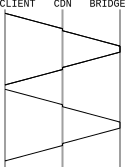
\includegraphics[width=\linewidth]{wire-sequential}
\caption{Sequential}
\label{fig:wire-sequential}
\end{subfigure}
\qquad
\begin{subfigure}[t]{0.40\linewidth}
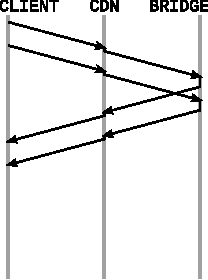
\includegraphics[width=\linewidth]{wire-parallel}
\caption{Parallel}
\label{fig:wire-parallel}
\end{subfigure}

\caption{
The nature of potential performance gain
from sending fronted requests in parallel.
}
\label{fig:wire}
\end{figure}

We have assumed that the intermediate web service is
outside the censor's domain of control,
so that communication between the web service and Tor bridge
doesn't have to be protected.
What happens when the web service---a CDN edge server, for instance---is
inside the network controlled by the censor?
If the edge server forwards the request to the bridge
as an ordinary HTTP request on the public Internet,
then blocking it is as easy as blocking the IP address of the bridge.
On the other hand, if the web service encapsulates
the request and sends it encrypted, or over its own fast private network,
to another server outside of the censor's control,
then fronting will still work.

The ``domainless'' fronting style, which omits SNI,
is useful when there is no good front domain known for a web service.
At least one CDN, Fastly, requires the domainless style.
All current web browsers support SNI,
so it is possible that lack of SNI could be used as a distinguisher.
According to our communication with
a representative of
[a blinded organization observing many TLS connections],
% ANON
% the International Computer Science Institute's
% certificate notary~\cite{icsi-notary},
% which observes on the order of 50~million TLS connections daily,
83.5\% of connections used SNI in June~2014.
There are apparently enough connections without SNI
that a censor will at least have to consider seriously
the costs and benefits before deciding to block SNI-less TLS outright.

The current implementation of \meek\ strictly serializes
its HTTPS requests and responses,
in order to keep chunks of the underlying TCP stream
in the proper order.
The unfortunate side effect of this simple approach
is added latency that gets worse with longer round-trip times.
In future work we plan to add an additional reliability layer,
perhaps like the system of sequence numbers and acknowledgments used in OSS~\cite{oss},
that would allow requests to be pipelined
and cope with out-of-order delivery.
Figure~\ref{fig:wire-sequential} shows how the current implementation works,
and Figure~\ref{fig:wire-parallel} shows the nature of the performance
improvement that could be gained with a reliability layer
and parallel requests.
% Would be useful for Iran-like session cutoff, independent of \meek.

\meek's use of HTTPS is subject to the usual public key infrastructure
and trust model.
The browser running the HTTPS camouflage extension (Section~\ref{sec:browserextension})
has a list of trusted certificate authorities.
A censor that controls a certificate authority trusted by the browser
is able to perform a man-in-the-middle attack
between the client and the intermediate web service,
and detect fronting by decrypting TLS and checking for specific Host headers.
Such a censor would be able to detect circumvention,
but still not read the client's plaintext because of the
additional encryption and authentication of the tunneled Tor layer.
It seems risky for the censor to risk being detected in
a man-in-the-middle attack merely to confirm that a user is circumventing,
but it is not impossible for a sufficiently powerful censor.
The problem doesn't exist when the front domain is one
that happens have its public key ``pinned'' in the headless browser,
for instance when using the Chrome extension and fronting through
\urll{www.google.com}.

% \meek\ apart from Tor.
% more risk for the proxy operator
% can require people to run their own proxies à la GoAgent.
% "Censorship implies surveillance"

The key idea of \meek\ is domain fronting,
but its HTTP tunneling ability is useful on its own.
Another idea for deployment is to use
thousands of simple HTTP reflectors on cheap web hosting
(in place of domain fronting on a big CDN).
The request-reflecting role of a CDN can
be played by a PHP script, for example,
or a special web server configuration.
Their URLs unprotected by domain fronting,
each reflector would be easily blockable individually,
so there would need to be sufficiently many that
a censor could not block them all.
This deployment model is essentially the same as with
ordinary Tor bridges: have lots of volunteer-operated bridges
and make it hard to enumerate them all.
The advantage that an HTTP transport would have
is that it is easier for a volunteer to upload a PHP file to a web host
than to set up and maintain a Tor bridge.

\section{Summary}
\label{sec:summary}

We have presented domain fronting,
an HTTPS technique that uses different domain names
at different communication layers in
order to hide the remote endpoint of a communication.
We implemented \meek,
a pluggable transport for Tor.
We show that it resists common methods of blocking,
and begin an investigation into its
resistance against more subtle and expensive means of traffic analysis.
We discuss the results of an initial deployment.
% ANON
% in both Tor and Psiphon.

[Links to source code omitted for anonymous submission.]
% ANON
% \meek\ has a home page at
% \url{https://trac.torproject.org/projects/tor/wiki/doc/meek}.
% Our source code is in the Git repository at
% \url{https://git.torproject.org/pluggable-transports/meek.git}.
% All our programs are free software.

% As of version 0.9 (June~19, 2014), the source code consists of
% about 1,100 lines of Go for the client programs,
% 400 lines for \meekserver, and
% 100 lines for the reflector application for App Engine.
% Each of the browser extensions
% (one for Firefox, one for Chrome)
% is about 400 lines of JavaScript.

% ANON
% \section*{Acknowledgments}

% We thank Vern Paxson, Nick Weaver, and Doug Tygar for inspiring conversation on this topic.
% Special thanks go to the members of the tor-qa and tor-dev mailing lists
% who responded to our design ideas, reviewed source code, and tested our prototypes.
% Thanks to Psiphon~Inc. for help with design and development, and for providing user count estimates.
% George Kadianakis
% Georg Koppen
% Lunar
% Yawning Angel
% Ox from Lantern.
% Johanna Amann for getting the fraction of SNI from ICSI notary:
%   https://trac.torproject.org/projects/tor/ticket/12208#comment:5
% Arlo Breault (flashproxy-reg-appspot)
% Sadia Afroz and Michael Tschantz

%%%%%%%

% HTTPS or not on the App Engine--bridge link.
% HTTPS obscures session ids, equivalent to obscuring TCP connections in other transports.
% Increases latency a lot: \approx 100 ms increased to \approx 350 ms when I tried it in March 2014.

\bibliographystyle{abbrv}
\bibliography{meek}

\appendix

\section{Sample TLS fingerprints}
\label{sec:ciphersuites}

\begin{figure*}
\centering
\begin{subfigure}[t]{0.30\textwidth}
\caption{Go 1.2's crypto/tls library}
\begin{minipage}[t][25.5ex][t]{\textwidth}
\tiny
\begin{verbatim}
Ciphersuites:
  TLS_ECDHE_RSA_WITH_AES_128_GCM_SHA256
  TLS_ECDHE_ECDSA_WITH_AES_128_GCM_SHA256
  TLS_ECDHE_RSA_WITH_RC4_128_SHA
  TLS_ECDHE_ECDSA_WITH_RC4_128_SHA
  TLS_ECDHE_RSA_WITH_AES_128_CBC_SHA
  TLS_ECDHE_ECDSA_WITH_AES_128_CBC_SHA
  TLS_ECDHE_RSA_WITH_AES_256_CBC_SHA
  TLS_ECDHE_ECDSA_WITH_AES_256_CBC_SHA
  TLS_RSA_WITH_RC4_128_SHA
  TLS_RSA_WITH_AES_128_CBC_SHA
  TLS_RSA_WITH_AES_256_CBC_SHA
  TLS_ECDHE_RSA_WITH_3DES_EDE_CBC_SHA
  TLS_RSA_WITH_3DES_EDE_CBC_SHA
Extensions:
  server_name
  status_request
  elliptic_curves
  ec_point_formats
  signature_algorithms
\end{verbatim}
\end{minipage}
\label{fig:ciphersuites:golang}
\end{subfigure}
%
\begin{subfigure}[t]{0.30\textwidth}
\caption{Firefox 24}
\begin{minipage}[t][65ex][t]{\textwidth}
\tiny
\begin{verbatim}
Ciphersuites:
  TLS_ECDHE_ECDSA_WITH_AES_256_CBC_SHA
  TLS_ECDHE_ECDSA_WITH_AES_128_CBC_SHA
  TLS_ECDHE_RSA_WITH_AES_128_CBC_SHA
  TLS_ECDHE_RSA_WITH_AES_256_CBC_SHA
  TLS_ECDHE_ECDSA_WITH_3DES_EDE_CBC_SHA
  TLS_ECDHE_RSA_WITH_3DES_EDE_CBC_SHA
  TLS_ECDHE_ECDSA_WITH_RC4_128_SHA
  TLS_ECDHE_RSA_WITH_RC4_128_SHA
  TLS_DHE_RSA_WITH_AES_128_CBC_SHA
  TLS_DHE_DSS_WITH_AES_128_CBC_SHA
  TLS_DHE_RSA_WITH_CAMELLIA_128_CBC_SHA
  TLS_DHE_DSS_WITH_CAMELLIA_128_CBC_SHA
  TLS_DHE_RSA_WITH_AES_256_CBC_SHA
  TLS_DHE_DSS_WITH_AES_256_CBC_SHA
  TLS_DHE_RSA_WITH_CAMELLIA_256_CBC_SHA
  TLS_DHE_DSS_WITH_CAMELLIA_256_CBC_SHA
  TLS_DHE_RSA_WITH_3DES_EDE_CBC_SHA
  TLS_DHE_DSS_WITH_3DES_EDE_CBC_SHA
  TLS_ECDH_ECDSA_WITH_AES_128_CBC_SHA
  TLS_ECDH_RSA_WITH_AES_128_CBC_SHA
  TLS_ECDH_ECDSA_WITH_AES_256_CBC_SHA
  TLS_ECDH_RSA_WITH_AES_256_CBC_SHA
  TLS_ECDH_ECDSA_WITH_3DES_EDE_CBC_SHA
  TLS_ECDH_RSA_WITH_3DES_EDE_CBC_SHA
  TLS_ECDH_ECDSA_WITH_RC4_128_SHA
  TLS_ECDH_RSA_WITH_RC4_128_SHA
  TLS_RSA_WITH_AES_128_CBC_SHA
  TLS_RSA_WITH_CAMELLIA_128_CBC_SHA
  TLS_RSA_WITH_AES_256_CBC_SHA
  TLS_RSA_WITH_CAMELLIA_256_CBC_SHA
  TLS_RSA_WITH_SEED_CBC_SHA
  SSL_RSA_FIPS_WITH_3DES_EDE_CBC_SHA
  TLS_RSA_WITH_3DES_EDE_CBC_SHA
  TLS_RSA_WITH_RC4_128_SHA
  TLS_RSA_WITH_RC4_128_MD5
Extensions:
  server_name
  renegotiation_info
  elliptic_curves
  ec_point_formats
  SessionTicket TLS
  next_protocol_negotiation
\end{verbatim}
\end{minipage}
\label{fig:ciphersuites:firefox}
\end{subfigure}
%
\begin{subfigure}[t]{0.30\textwidth}
\caption{Chrome 33}
\begin{minipage}[t][42.5ex][t]{\textwidth}
\tiny
\begin{verbatim}
Ciphersuites:
  TLS_ECDHE_ECDSA_WITH_AES_128_GCM_SHA256
  TLS_ECDHE_RSA_WITH_AES_128_GCM_SHA256
  TLS_DHE_RSA_WITH_AES_128_GCM_SHA256
  TLS_ECDHE_ECDSA_WITH_CHACHA20_POLY1305_SHA256
  TLS_ECDHE_RSA_WITH_CHACHA20_POLY1305_SHA256
  TLS_RSA_WITH_AES_128_GCM_SHA256
  TLS_ECDHE_ECDSA_WITH_AES_256_CBC_SHA
  TLS_ECDHE_RSA_WITH_AES_256_CBC_SHA
  TLS_DHE_RSA_WITH_AES_256_CBC_SHA
  TLS_RSA_WITH_AES_256_CBC_SHA
  TLS_ECDHE_ECDSA_WITH_RC4_128_SHA
  TLS_ECDHE_ECDSA_WITH_AES_128_CBC_SHA
  TLS_ECDHE_RSA_WITH_RC4_128_SHA
  TLS_ECDHE_RSA_WITH_AES_128_CBC_SHA
  TLS_DHE_RSA_WITH_AES_128_CBC_SHA
  TLS_DHE_DSS_WITH_AES_128_CBC_SHA
  TLS_RSA_WITH_RC4_128_SHA
  TLS_RSA_WITH_RC4_128_MD5
  TLS_RSA_WITH_AES_128_CBC_SHA
  TLS_RSA_WITH_3DES_EDE_CBC_SHA
Extensions:
  server_name
  renegotiation_info
  elliptic_curves
  ec_point_formats
  SessionTicket TLS
  next_protocol_negotiation
  application_layer_protocol_negotiation
  Channel ID
  status_request
  signature_algorithms
  Signed Certificate Timestamp
\end{verbatim}
\end{minipage}
\label{fig:ciphersuites:chrome}
\end{subfigure}

\caption{
Selected differences in ClientHello messages in three different TLS implementations.
This figure illustrates the need for camouflage at the TLS layer.
Even though the TLS application data is effectively hidden by encryption,
the plaintext parts of TLS reveal information about the implementation.
The TLS must not be easily identified as belonging to a circumvention tool.
}
\label{fig:ciphersuites}
\end{figure*}

\end{document}
